% chapters/03_hardware_design.tex - Chapter 3: Hardware Design
% =============================================================

\chapter{Mechanical \& Electrical Design}
\label{chap:hardware-design}

This chapter describes the hardware components, electrical systems, and physical assembly of the Rescue Rover. The design prioritizes modularity, repairability, and use of readily available components. Each subsystem is documented with specifications, selection rationale, and integration considerations.

% --------------------------------------------------------
% --------------------------------------------------------
% SECTION 3.1: DESIGN PHILOSOPHY
% --------------------------------------------------------
\section{Design Philosophy}
\label{sec:design-philosophy}

The hardware design follows three guiding principles. First, all components must be purchasable from common suppliers without lead times. Second, the system must be repairable using basic tools and without specialized equipment. Third, interfaces between modules must use standard connectors and protocols to allow future upgrades.

These constraints led us to select development boards over custom PCBs, through-hole components over surface mount where possible, and dupont wire connections over soldered joints for early prototypes.

% FIGURE 3.1: ROVER PHOTO
% Placed inside Section 3.1
\begin{figure}[H]
    \centering
    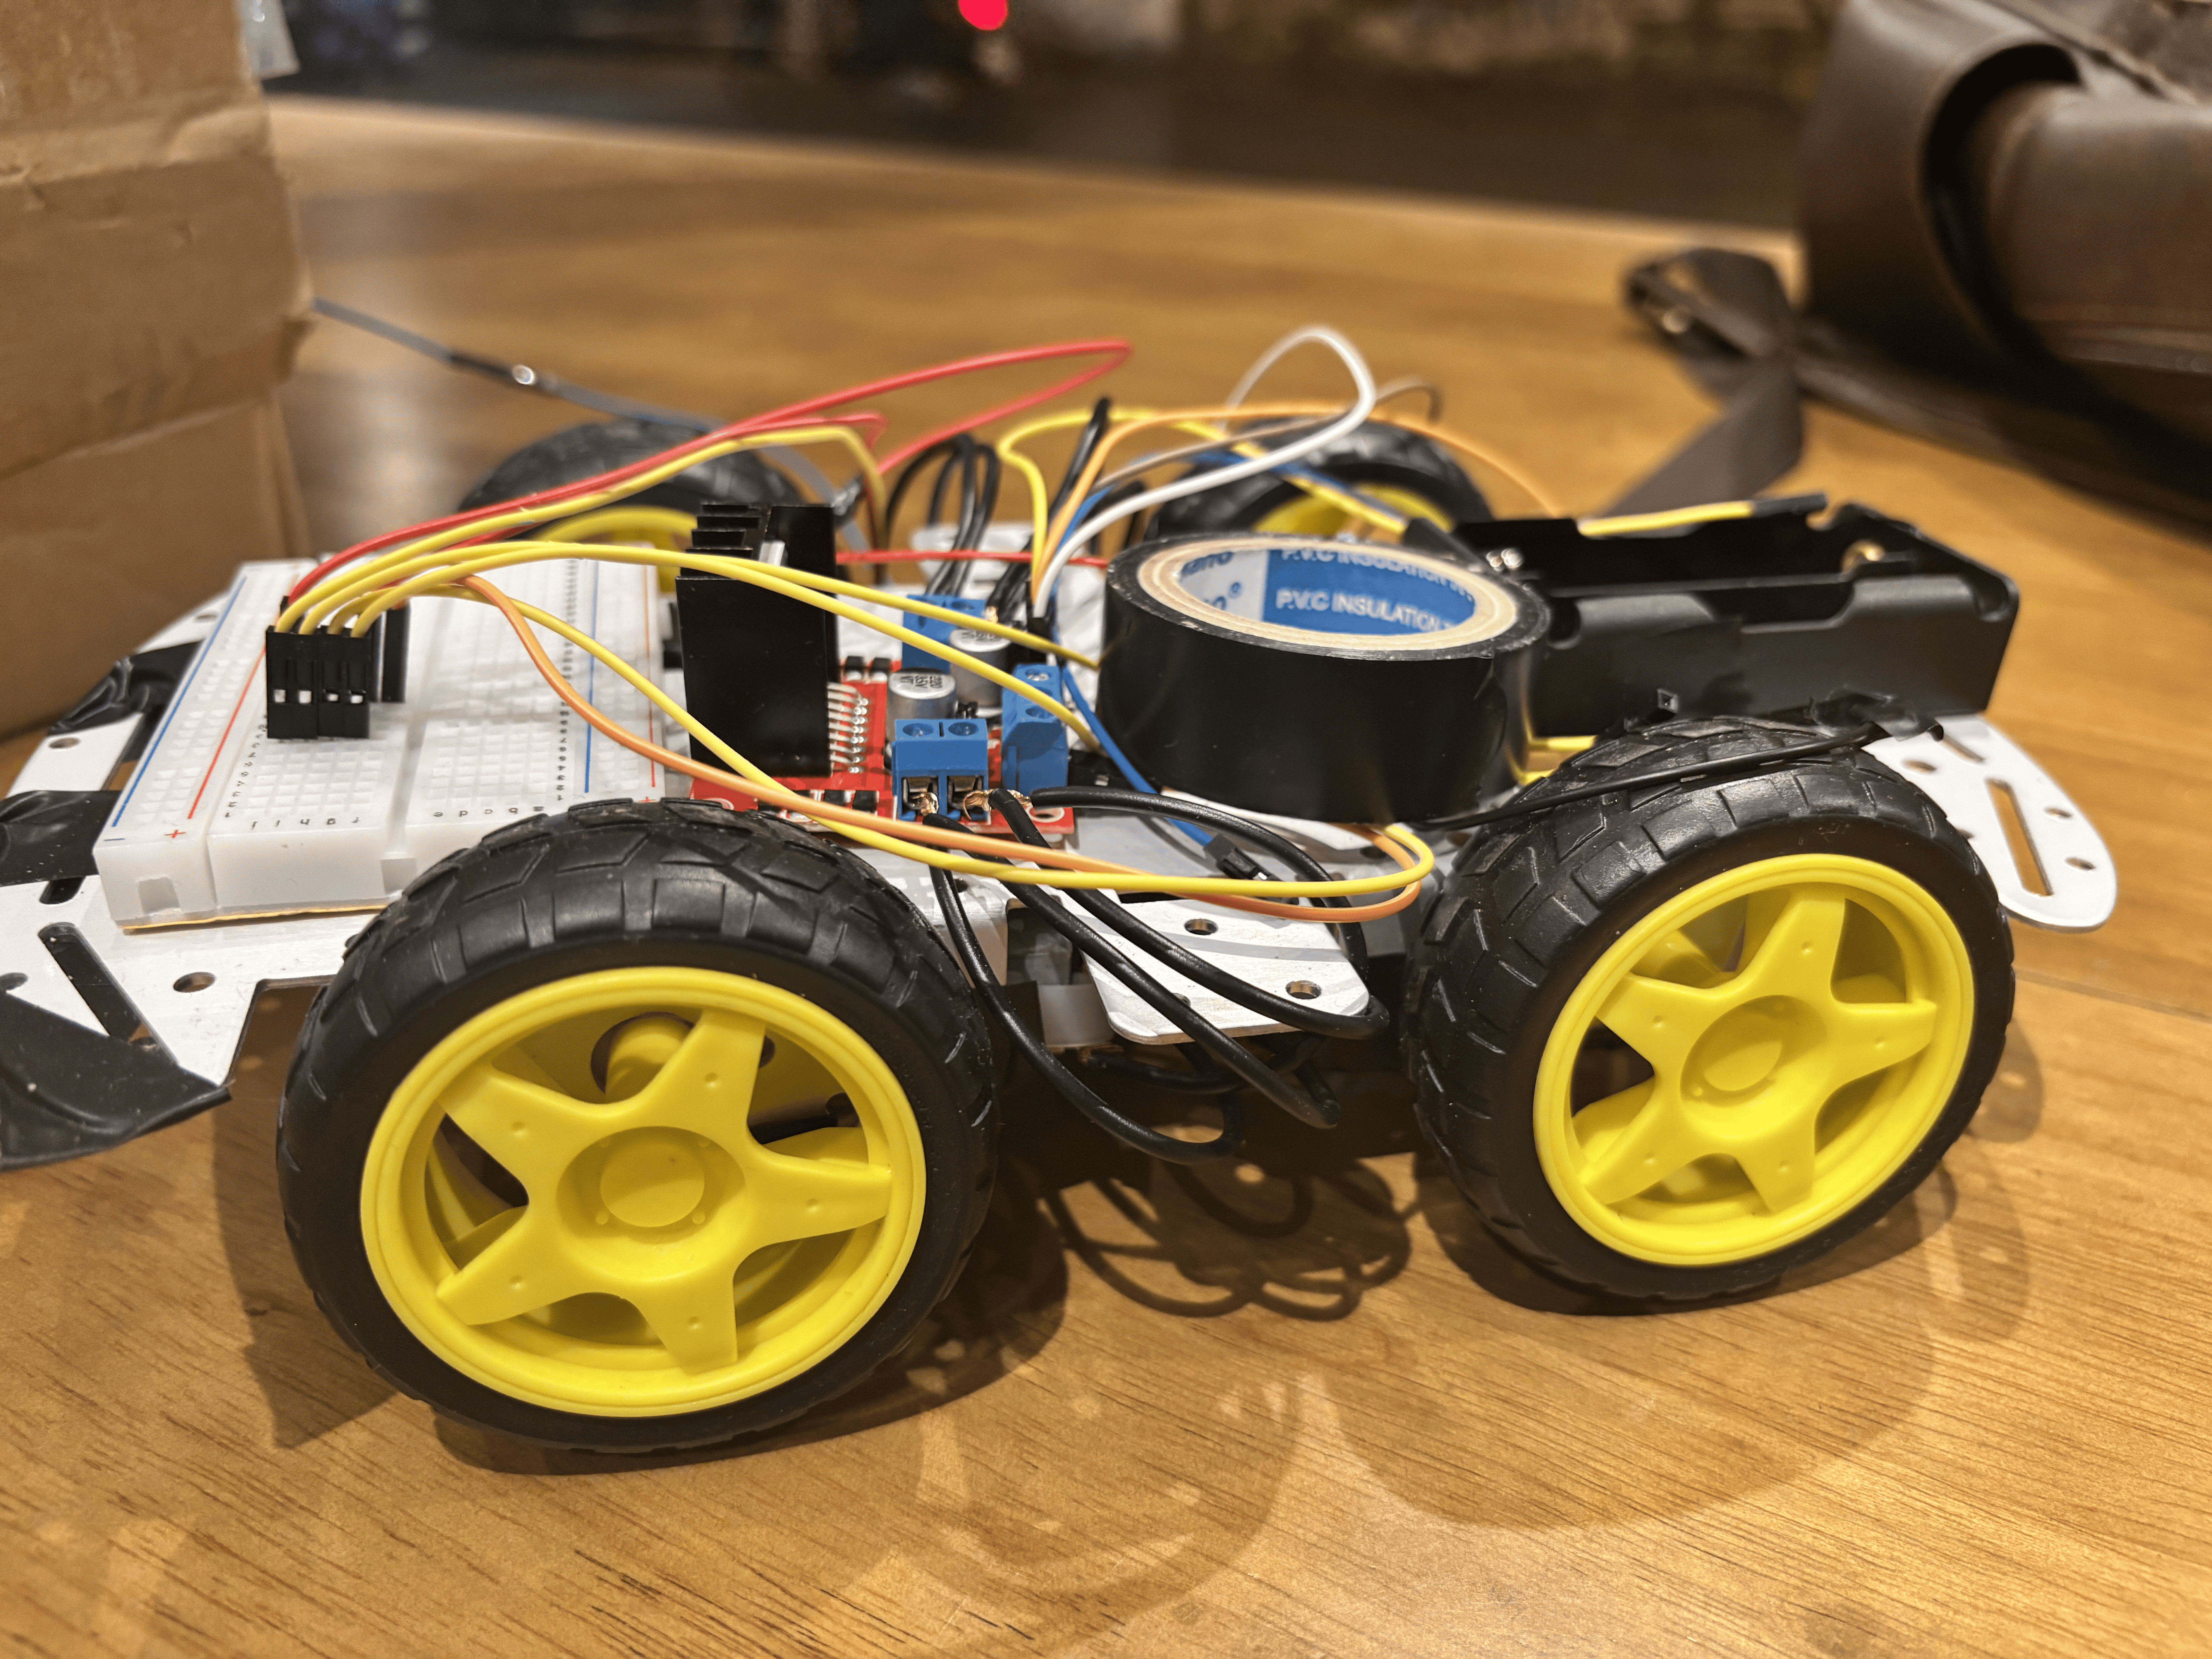
\includegraphics[width=\textwidth]{figures/hardware/rover_complete_photo.png}
    \caption{Fully assembled Rescue Rover showing the ESP32-S3 camera module, motor driver, battery, and chassis.}
    \label{fig:rover-complete}
\end{figure}

% --------------------------------------------------------
% SECTION 3.2: CHASSIS DESIGN
% --------------------------------------------------------
\section{Chassis Design}
\label{sec:chassis-design}

The chassis provides the structural foundation for all electronic components. We selected a commercially available \textbf{4-wheel drive (4WD)} chassis platform rather than designing a custom frame. This decision saved significant development time while providing a proven mechanical platform for the rover.

% SUBSECTION 3.2.1: PLATFORM SELECTION
\subsection{Platform Selection}

The selected chassis is a \textbf{dual-layer acrylic smart car platform}. Unlike the tracked tank-style alternatives initially considered, this wheeled design was chosen for its kinematic simplicity, higher top speed on flat surfaces, and easier maintenance. The acrylic construction allows for rapid modification and flexible component mounting.

\begin{table}[h!]
    \centering
    \caption{Chassis specifications (4WD Wheel Platform)}
    \label{tab:chassis-specs}
    \begin{tabular}{ll}
        \toprule
        \textbf{Parameter} & \textbf{Value} \\
        \midrule
        Drive System & 4-Wheel Drive (Independent DC Motors) \\
        Dimensions (L x W) & 255mm x 150mm (Chassis Plate) \\
        Full Width & $\approx$ 210mm (with wheels) \\
        Material & Laser-cut Acrylic \\
        Wheel Diameter & 65mm (Rubber tires) \\
        Motor Type & 1:48 Gear Ratio TT Motors \\
        \bottomrule
    \end{tabular}
\end{table}

% FIGURE 3.2: CHASSIS DIMENSIONS
% Placed inside Subsection 3.2.1
\begin{figure}[H]
    \centering
    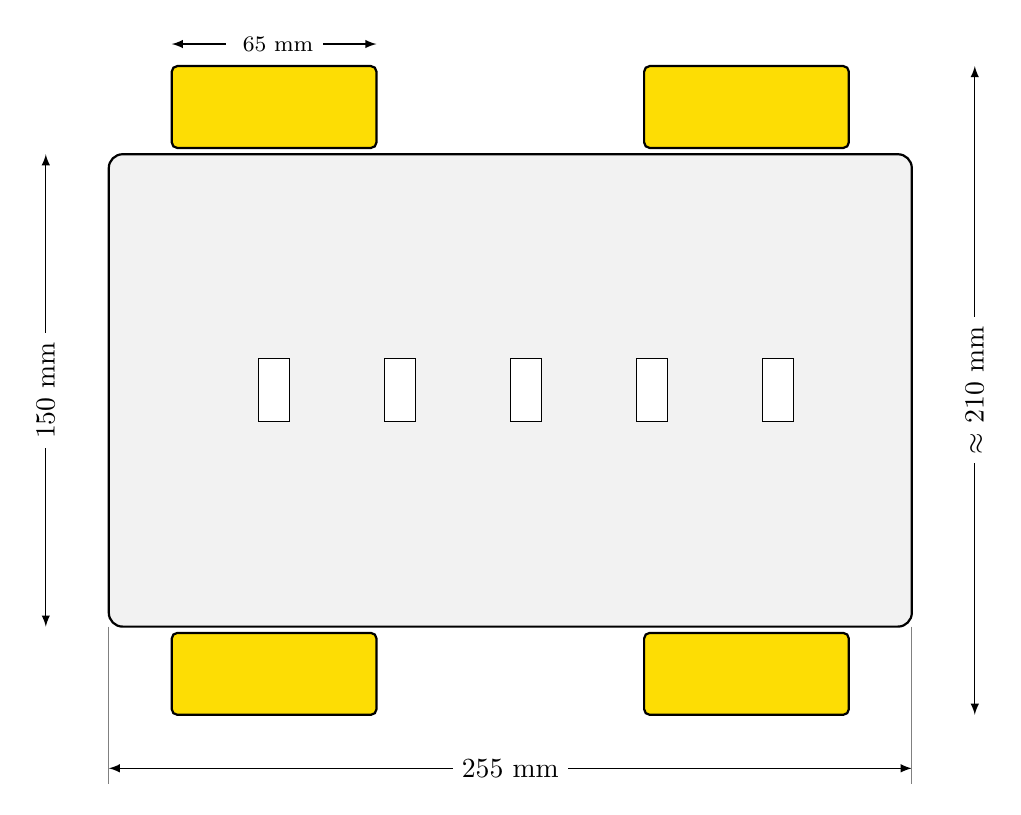
\begin{tikzpicture}[scale=0.04] 
        % Definitions
        \def\chassisL{255} 
        \def\chassisW{150} 
        \def\wheelL{65}    
        \def\wheelW{26}    

        % Styles
        \tikzstyle{dim} = [draw, <->, >=latex, thin, black]
        \tikzstyle{line} = [draw, thick, black]
        \tikzstyle{part} = [fill=gray!10, draw=black, thick]
        \tikzstyle{wheel} = [fill=yellow!80!orange, draw=black, thick, rounded corners=2pt]

        % Chassis
        \draw[part, rounded corners=5pt] (-\chassisL/2, -\chassisW/2) rectangle (\chassisL/2, \chassisW/2);
        \foreach \x in {-80, -40, 0, 40, 80} {
            \draw[fill=white] (\x, -10) rectangle (\x+10, 10);
        }

        % Wheels
        \draw[wheel] (-\chassisL/2 + 20, \chassisW/2 + 2) rectangle ++(\wheelL, \wheelW);
        \draw[wheel] (-\chassisL/2 + 20, -\chassisW/2 - 2 - \wheelW) rectangle ++(\wheelL, \wheelW);
        \draw[wheel] (\chassisL/2 - 20 - \wheelL, \chassisW/2 + 2) rectangle ++(\wheelL, \wheelW);
        \draw[wheel] (\chassisL/2 - 20 - \wheelL, -\chassisW/2 - 2 - \wheelW) rectangle ++(\wheelL, \wheelW);

        % Dimensions
        \draw[dim] (-\chassisL/2, -\chassisW/2 - 45) -- (\chassisL/2, -\chassisW/2 - 45) node[midway, fill=white] {255 mm};
        \draw[line, thin, gray] (-\chassisL/2, -\chassisW/2) -- (-\chassisL/2, -\chassisW/2 - 50);
        \draw[line, thin, gray] (\chassisL/2, -\chassisW/2) -- (\chassisL/2, -\chassisW/2 - 50);
        \draw[dim] (\chassisL/2 + 20, -\chassisW/2 - \wheelW - 2) -- (\chassisL/2 + 20, \chassisW/2 + \wheelW + 2) node[midway, fill=white, rotate=90] {$\approx$ 210 mm};
        \draw[dim] (-\chassisL/2 - 20, -\chassisW/2) -- (-\chassisL/2 - 20, \chassisW/2) node[midway, fill=white, rotate=90] {150 mm};
        \draw[dim] (-\chassisL/2 + 20, \chassisW/2 + 35) -- (-\chassisL/2 + 20 + \wheelL, \chassisW/2 + 35) node[midway, fill=white, font=\footnotesize] {$\varnothing$ 65 mm};

    \end{tikzpicture}
    \caption{Top-down dimensional schematic of the 4WD Rover chassis. The platform utilizes a double-layer acrylic frame with four independently driven DC geared motors.}
    \label{fig:chassis-dimensions}
\end{figure}

% SUBSECTION 3.2.2: WHEEL AND DRIVE ASSEMBLY
\subsection{Wheel and Drive Assembly}
\label{sec:drive-assembly}

Instead of the complex track tensioning system initially proposed, the rover utilizes a direct-drive configuration. Each of the four wheels is mounted directly to the output shaft of a DC gear motor. The system uses standard "TT" style motors with a 1:48 gear ratio. The wheels ($65\text{mm}$ diameter) feature a solid plastic rim with a rubber tire for traction. Torque is transferred via a double-flat mechanical interface that prevents the wheel from slipping on the motor shaft, eliminating the need for belts or tensioners.

% FIGURE 3.3: MOTOR DETAIL
% Placed inside Subsection 3.2.2
\begin{figure}[H]
    \centering
    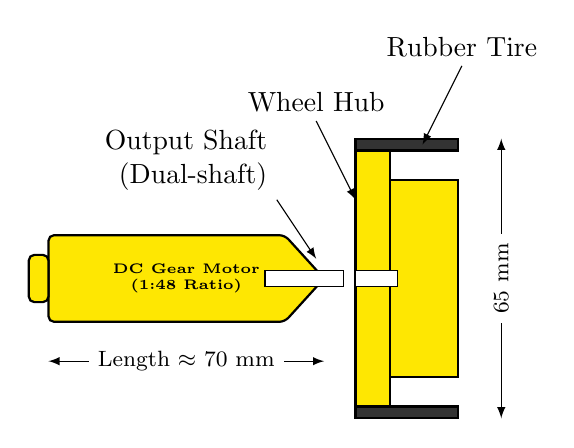
\begin{tikzpicture}[scale=0.05, >=latex]

        % Styles
        \tikzstyle{motor} = [draw=black, thick, fill=yellow!90!orange, rounded corners=2pt]
        \tikzstyle{tire} = [draw=black, fill=black!80, thick]
        \tikzstyle{rim} = [draw=black, fill=yellow!90!orange, thick]
        \tikzstyle{shaft} = [draw=black, fill=white]
        \tikzstyle{label} = [midway, fill=white, font=\footnotesize]
        \tikzstyle{dim} = [draw, <->, thin, black]

        % Definitions
        \def\motorL{70}
        \def\motorH{22}
        \def\wheelDia{65}
        \def\wheelW{26}

        % Drawing
        \draw[motor] (0, 0) -- (0, \motorH) -- (\motorL-10, \motorH) -- (\motorL, \motorH/2) -- (\motorL-10, 0) -- cycle;
        \draw[motor] (-5, 5) rectangle (0, \motorH-5);
        \node at (\motorL/2, \motorH/2) [font=\bfseries\tiny, align=center] {DC Gear Motor\\(1:48 Ratio)};

        \draw[shaft] (\motorL-15, \motorH/2 - 2) rectangle (\motorL+5, \motorH/2 + 2);

        \begin{scope}[shift={(\motorL+8, \motorH/2)}]
            \draw[tire] (0, \wheelDia/2) rectangle (\wheelW, \wheelDia/2 + 3); 
            \draw[tire] (0, -\wheelDia/2) rectangle (\wheelW, -\wheelDia/2 - 3); 
            \draw[rim] (0, -\wheelDia/2) rectangle (\wheelW/3, \wheelDia/2); 
            \draw[rim] (\wheelW/3, -25) rectangle (\wheelW, 25); 
            \draw[fill=white] (0, -2) rectangle (\wheelW/3 + 2, 2);
        \end{scope}

        % Dimensions
        \draw[dim] (\motorL+45, \motorH/2 - \wheelDia/2 - 3) -- (\motorL+45, \motorH/2 + \wheelDia/2 + 3) node[label, rotate=90] {$\varnothing 65$ mm};
        \draw[dim] (0, -10) -- (\motorL, -10) node[label] {Length $\approx$ 70 mm};

        % Annotations
        \draw[<-] (\motorL+8, \motorH/2 + 20) -- ++(-10, 20) node[anchor=south] {Wheel Hub};
        \draw[<-] (\motorL+25, \motorH/2 + 34) -- ++(10, 20) node[anchor=south] {Rubber Tire};
        \draw[<-] (\motorL-2, \motorH/2 + 5) -- ++(-10, 15) node[anchor=south east, align=right] {Output Shaft\\(Dual-shaft)};

    \end{tikzpicture}
    \caption{Drive assembly detail. The 1:48 ratio DC Gear Motor (left) couples directly to the 65mm wheel (right). The yellow plastic rim is press-fitted onto the motor output shaft.}
    \label{fig:drive-detail}
\end{figure}

\subsection{Component Mounting}
Electronic components are secured to the acrylic chassis to ensure stability during operation. The main PCB modules, such as the ESP32-S3 and the L298N motor driver, are mounted using \textbf{nylon standoffs and M3 screws}. This provides electrical isolation from the chassis and allows for easy removal. The prototyping breadboard is secured using a strong double-sided adhesive pad. Components are arranged longitudinally to distribute weight evenly between the front and rear axles, placing the heavier battery pack at the rear to counterbalance the camera and sensor array at the front.

% FIGURE PLACEHOLDER
\begin{figure}[H]
    \centering
    % FIX: Set x and y vectors to 1mm so "255" = 25.5cm, not 2.55 meters.
    % FIX: Scale 0.6 fits it nicely on a standard page width.
    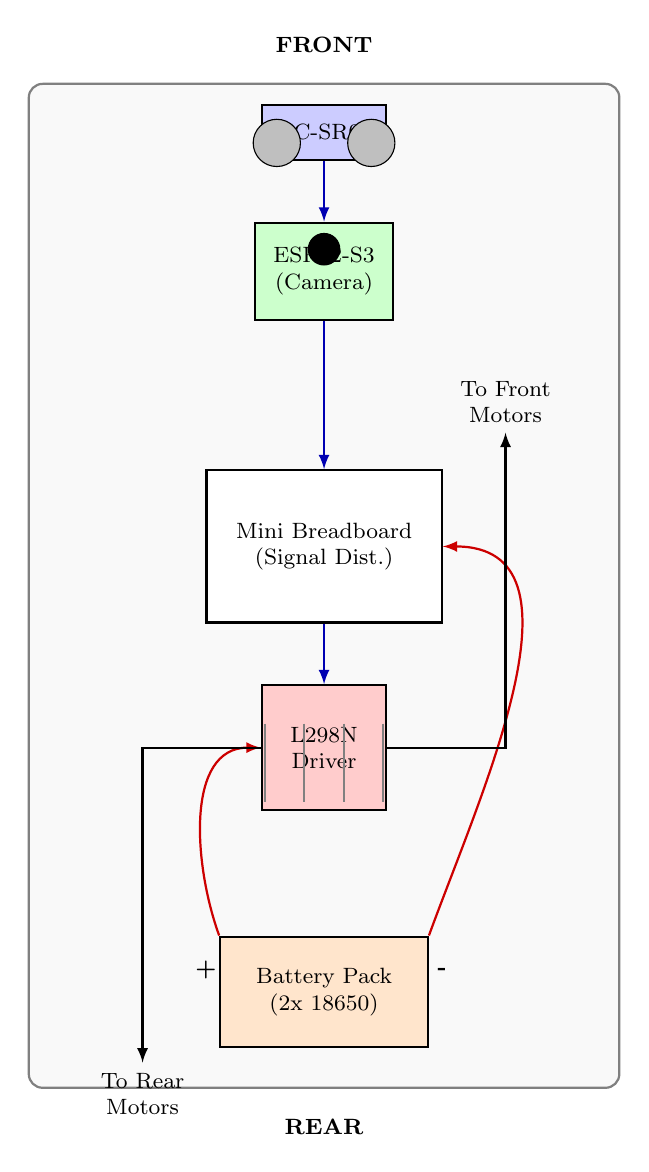
\begin{tikzpicture}[x=1mm, y=1mm, scale=0.5, >=latex, font=\footnotesize]

        % --- STYLES ---
        % FIX: Added 'align=center' to all nodes to allow line breaks (\\)
        \tikzstyle{chassis} = [draw=gray, thick, fill=gray!5, rounded corners=5pt]
        \tikzstyle{pcb_esp} = [draw=black, fill=green!20!white, thick, align=center]
        \tikzstyle{pcb_driver} = [draw=black, fill=red!20!white, thick, align=center]
        \tikzstyle{breadboard} = [draw=black, fill=white, thick, align=center] % Removed pattern to prevent errors
        \tikzstyle{sensor} = [draw=black, fill=blue!20!white, thick, align=center]
        \tikzstyle{battery} = [draw=black, fill=orange!20!white, thick, align=center]
        \tikzstyle{wire} = [draw=blue!70!black, thick, ->]
        \tikzstyle{label_node} = [fill=white, draw=black, thin, inner sep=2pt, align=center]

        % --- DEFINITIONS ---
        \def\cL{255} % Chassis Length (now interpreted as mm)
        \def\cW{150} % Chassis Width (now interpreted as mm)

        % --- CHASSIS BASE ---
        \draw[chassis] (-\cW/2, -\cL/2) rectangle (\cW/2, \cL/2);
        \node at (0, \cL/2 + 10) {\textbf{FRONT}};
        \node at (0, -\cL/2 - 10) {\textbf{REAR}};

        % --- COMPONENTS ---

        % 1. Ultrasonic Sensor (Front)
        \node[sensor, minimum width=45, minimum height=20, anchor=north] (us) at (0, \cL/2 - 5) {HC-SR04};
        % Add "eyes"
        \draw[fill=gray!50] (-12, \cL/2 - 15) circle (6);
        \draw[fill=gray!50] (12, \cL/2 - 15) circle (6);

        % 2. ESP32-S3 Camera Module (Behind sensor)
        \node[pcb_esp, minimum width=50, minimum height=35, anchor=north] (esp) at (0, \cL/2 - 35) {ESP32-S3\\(Camera)};
        % Add lens indication
        \draw[fill=black] (0, \cL/2 - 42) circle (4);

        % 3. Breadboard (Middle)
        \node[breadboard, minimum width=85, minimum height=55] (bb) at (0, 10) {Mini Breadboard\\(Signal Dist.)};

        % 4. L298N Motor Driver (Behind breadboard)
        \node[pcb_driver, minimum width=45, minimum height=45, anchor=north] (driver) at (0, -25) {L298N\\Driver};
        % Add heatsink graphic
        \foreach \x in {-15, -5, 5, 15} \draw[gray, thick] (\x, -35) -- (\x, -55);

        % 5. Battery Pack (Rear)
        \node[battery, minimum width=75, minimum height=40, anchor=south] (batt) at (0, -\cL/2 + 10) {Battery Pack\\(2x 18650)};
        % Add terminals
        \node at (-30, -\cL/2 + 30) {\textbf{+}};
        \node at (30, -\cL/2 + 30) {\textbf{-}};

        % --- LOGICAL CONNECTIONS (Schematic Wires) ---
        % Sensor to ESP
        \draw[wire] (us.south) -- (esp.north);
        % ESP to Breadboard
        \draw[wire] (esp.south) -- (bb.north);
        % Breadboard to Driver (Control signals)
        \draw[wire] (bb.south) -- (driver.north);
        
        % Battery to Driver (Power)
        % Note: Adjusted 'out' angle slightly to be smoother
        \draw[wire, draw=red!80!black] (batt.north west) to[out=110, in=180] (driver.west);
        
        % Battery to ESP (Power via regulator/breadboard)
        \draw[wire, draw=red!80!black] (batt.north east) to[out=70, in=0] (bb.east);

        % Motor outputs (schematic)
        \draw[wire, draw=black, thick] (driver.east) -- ++(30,0) -- ++(0, 80) node[above, align=center] {To Front\\Motors};
        \draw[wire, draw=black, thick] (driver.west) -- ++(-30,0) -- ++(0, -80) node[below, align=center] {To Rear\\Motors};

    \end{tikzpicture}
    \caption{Schematic top-down view of the component layout. The ultrasonic sensor and camera are positioned at the front for unobstructed sensing. The heavier battery pack is placed at the rear to balance the center of gravity. Power and signal lines are shown logically.}
    \label{fig:component-layout}
\end{figure}

% --------------------------------------------------------
\section{Main Controller: ESP32-S3}
\label{sec:esp32-controller}

The ESP32-S3 serves as the central processing unit for the rover. This chip was selected for its combination of processing power, wireless capabilities, camera interface, and extensive Arduino ecosystem support.

\subsection{Chip Specifications}

The ESP32-S3 is Espressif's third generation WiFi/Bluetooth microcontroller. It features dual Xtensa LX7 cores running at up to 240 MHz, significantly more powerful than the original ESP32.

\begin{table}[H]
    \centering
    \caption{ESP32-S3 technical specifications}
    \label{tab:esp32-specs}
    \begin{tabular}{ll}
        \toprule
        \textbf{Feature} & \textbf{Specification} \\
        \midrule
        CPU           & Dual Xtensa LX7, up to 240 MHz \\
        SRAM          & 512 KB internal \\
        PSRAM         & 8 MB external (OPI interface) \\
        Flash         & 16 MB (QSPI) \\
        WiFi          & 802.11 b/g/n, 2.4 GHz \\
        Bluetooth     & LE 5.0 with coded PHY \\
        GPIO          & 45 programmable pins \\
        Camera        & DVP interface, up to 2MP \\
        USB           & USB 2.0 OTG \\
        Operating voltage & 3.0-3.6V (LDO regulates from 5V)\\
        \bottomrule
    \end{tabular}
\end{table}

% FIGURE PLACEHOLDER
\begin{figure}[H]
    \centering
    \includegraphics[width=0.7\textwidth]{figures/hardware/esp32s3_module_photo.jpeg}
    \caption{ESP32-S3 WROOM development board used in the Rescue Rover.}
    \label{fig:esp32-module}
\end{figure}

\subsection{Development Board Selection}

Several ESP32-S3 development boards were evaluated. The Freenove ESP32-S3 WROOM was selected for its integrated camera connector, adequate PSRAM, and reasonable price point. Other options considered included the official Espressif DevKitC and the AI-Thinker ESP32-S3 CAM.

\begin{table}[H]
    \centering
    \caption{ESP32-S3 development board comparison}
    \label{tab:board-comparison}
    \begin{tabular}{lccc}
        \toprule
        \textbf{Feature} & \textbf{Freenove} & \textbf{ESP32-CAM} & \textbf{DevKitC} \\
        \midrule
        PSRAM             & 8 MB  & 4 MB  & 8 MB \\
        Camera connector  & Yes   & Yes   & No \\
        Available GPIO    & 35+   & 10    & 45 \\
        USB programming   & Built-in & External & Built-in \\
        Price             & \$12  & \$8   & \$15 \\
        Selected          & Yes   & No    & No \\
        \bottomrule
    \end{tabular}
\end{table}

The ESP32-CAM was rejected despite its lower cost because of severe GPIO limitations. Many pins are shared between the camera, SD card, and flash, leaving insufficient pins for motor control and sensors.

% FIGURE PLACEHOLDER
% FIGURE: BOARD COMPARISON
\begin{figure}[H]
    \centering
    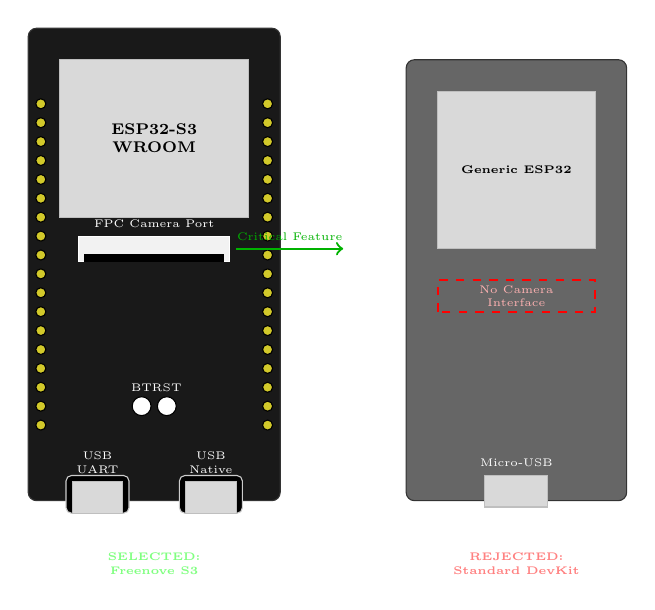
\begin{tikzpicture}[scale=0.8, transform shape, font=\sffamily\footnotesize]

        % Styles
        \tikzstyle{pcb} = [draw=black!80, fill=black!90, rounded corners=3pt]
        \tikzstyle{metal} = [draw=gray!50, fill=gray!30]
        \tikzstyle{conn} = [draw=white, fill=white!90!gray]
        \tikzstyle{usbc} = [draw=gray!40, fill=black, rounded corners=2pt]
        \tikzstyle{label} = [text=white, font=\bfseries\tiny, align=center]
        
        % --- LEFT: FREENOVE S3 (SELECTED) ---
        \begin{scope}[shift={(0,0)}]
            % PCB Outline
            \draw[pcb] (0,0) rectangle (4.0, 7.5);
            
            % ESP32-S3 Module
            \draw[metal] (0.5, 4.5) rectangle (3.5, 7.0);
            \node[text=black, font=\bfseries\scriptsize, align=center] at (2.0, 5.75) {ESP32-S3\\WROOM};

            % FPC Camera Connector (The distinctive white bar)
            \draw[conn] (0.8, 3.8) rectangle (3.2, 4.2);
            \draw[black, fill=black] (0.9, 3.8) rectangle (3.1, 3.9); % Latch
            \node[text=white, font=\tiny] at (2.0, 4.4) {FPC Camera Port};

            % Dual USB-C Ports (Bottom)
            \draw[usbc] (0.6, -0.2) rectangle (1.6, 0.4); % UART
            \draw[metal] (0.7, -0.2) rectangle (1.5, 0.3); % Metal casing
            \node[text=white, font=\tiny, align=center] at (1.1, 0.6) {USB\\UART};

            \draw[usbc] (2.4, -0.2) rectangle (3.4, 0.4); % OTG
            \draw[metal] (2.5, -0.2) rectangle (3.3, 0.3); % Metal casing
            \node[text=white, font=\tiny, align=center] at (2.9, 0.6) {USB\\Native};

            % Header Pins
            \foreach \y in {1.2, 1.5, ..., 6.5} {
                \draw[fill=yellow!80!black] (0.2, \y) circle (0.08);
                \draw[fill=yellow!80!black] (3.8, \y) circle (0.08);
            }

            % Buttons (Boot/Rst)
            \draw[fill=white] (1.8, 1.5) circle (0.15); \node[text=white, font=\tiny] at (1.8, 1.8) {BT};
            \draw[fill=white] (2.2, 1.5) circle (0.15); \node[text=white, font=\tiny] at (2.2, 1.8) {RST};

            % Label
            \node[label, text=green!50] at (2.0, -1.0) {SELECTED:\\Freenove S3};
        \end{scope}

        % --- RIGHT: STANDARD DEVKIT (REJECTED) ---
        \begin{scope}[shift={(6,0)}]
            % PCB Outline
            \draw[pcb, fill=black!60] (0,0) rectangle (3.5, 7.0);
            
            % Module
            \draw[metal] (0.5, 4.0) rectangle (3.0, 6.5);
            \node[text=black, font=\bfseries\tiny] at (1.75, 5.25) {Generic ESP32};

            % NO Camera Port (Crossed out area)
            \draw[red, dashed, thick] (0.5, 3.0) rectangle (3.0, 3.5);
            \node[text=red!30, font=\tiny, align=center] at (1.75, 3.25) {No Camera\\Interface};

            % Single Micro-USB
            \draw[metal] (1.25, -0.1) rectangle (2.25, 0.4);
            \node[text=white, font=\tiny] at (1.75, 0.6) {Micro-USB};

            % Label
            \node[label, text=red!50] at (1.75, -1.0) {REJECTED:\\Standard DevKit};
        \end{scope}

        % --- COMPARISON ARROWS ---
        \draw[->, thick, green!70!black] (3.3, 4.0) -- (5.0, 4.0) node[midway, above, font=\tiny] {Critical Feature};

    \end{tikzpicture}
    \caption{Comparison of development boards. The Freenove S3 (left) was selected for its dedicated FPC camera connector and dual USB-C interfaces, features absent on standard development boards (right).}
    \label{fig:board-comparison}
\end{figure}

\subsection{PSRAM Importance}

External PSRAM is essential for camera operation. Each QVGA frame requires 153.6 KB of buffer space. Double buffering doubles this requirement. Without PSRAM, the internal 512 KB SRAM would be exhausted by camera buffers alone, leaving no memory for the application.

The PSRAM connects via OPI (Octal Peripheral Interface) rather than QPI (Quad). OPI provides higher bandwidth, supporting faster frame transfers from the camera peripheral to the CPU.

% --------------------------------------------------------
\section{Camera System}
\label{sec:camera-hardware}

The camera provides the rover's primary sensing capability. Visual data is used for remote operation, obstacle detection, and AI scene analysis.

\subsection{OV2640 Sensor}

The OV2640 is a 2-megapixel CMOS image sensor commonly used in embedded vision applications. It connects to the ESP32-S3 through the DVP (Digital Video Port) parallel interface.

\begin{table}[h!]
    \centering
    \caption{OV2640 camera sensor specifications}
    \label{tab:ov2640-specs}
    \begin{tabular}{ll}
        \toprule
        \textbf{Parameter} & \textbf{Value} \\
        \midrule
        Resolution (max)   & 1600 x 1200 (2 MP) \\
        Output formats     & JPEG, YUV422, RGB565 \\
        Frame rate (SVGA)  & 30 FPS \\
        Frame rate (UXGA)  & 15 FPS \\
        Interface          & DVP (8-bit parallel) \\
        Control bus        & I2C (SCCB compatible) \\
        Operating voltage  & 2.5V core, 2.8V I/O \\
        Active pixels      & 1632 x 1232 \\
        Pixel size         & 2.2 x 2.2 $\mu$m \\
        \bottomrule
    \end{tabular}
\end{table}

% FIGURE PLACEHOLDER
\begin{figure}[h!]
    \centering
    \includegraphics[width=0.5\textwidth]{figures/hardware/ov2640_module.jpeg}
    \caption{OV2640 camera module showing the lens assembly and 24-pin FPC connector.}
    \label{fig:ov2640-module}
\end{figure}

\subsection{Resolution Selection}
The firmware configures the OV2640 sensor for **QVGA ($320 \times 240$)** resolution. This specific setting was chosen as the optimal trade-off point. While the sensor supports up to UXGA ($1600 \times 1200$), resolutions above QVGA generate JPEG payloads that exceed the standard Ethernet MTU (1500 bytes), requiring complex UDP packet fragmentation and reassembly which increases latency.

\begin{table}[h!]
    \centering
    \caption{Resolution bandwidth trade-offs (OV2640 JPEG)}
    \label{tab:resolution-tradeoffs}
    \begin{tabular}{lcccc}
        \toprule
        \textbf{Resolution} & \textbf{Pixel Count} & \textbf{Avg Frame Size} & \textbf{UDP Efficiency} & \textbf{Status} \\
        \midrule
        QQVGA ($160\times120$) & 19,200    & 2-4 KB   & High (1 pkt) & Rejected (Low Detail) \\
        \textbf{QVGA ($320\times240$)}  & \textbf{76,800}    & \textbf{6-12 KB}  & \textbf{Medium (4-8 pkts)} & \textbf{Selected} \\
        VGA ($640\times480$)   & 307,200   & 25-40 KB & Low (20+ pkts)  & Rejected (High Latency) \\
        SVGA ($800\times600$)  & 480,000   & 50-80 KB & Very Low  & Rejected \\
        \bottomrule
    \end{tabular}
\end{table}

% FIGURE: RESOLUTION COMPARISON
\begin{figure}[h!]
    \centering
    % FIX: Set x and y to 0.2mm. 640 * 0.2mm = 128mm (12.8cm), which fits on the page.
    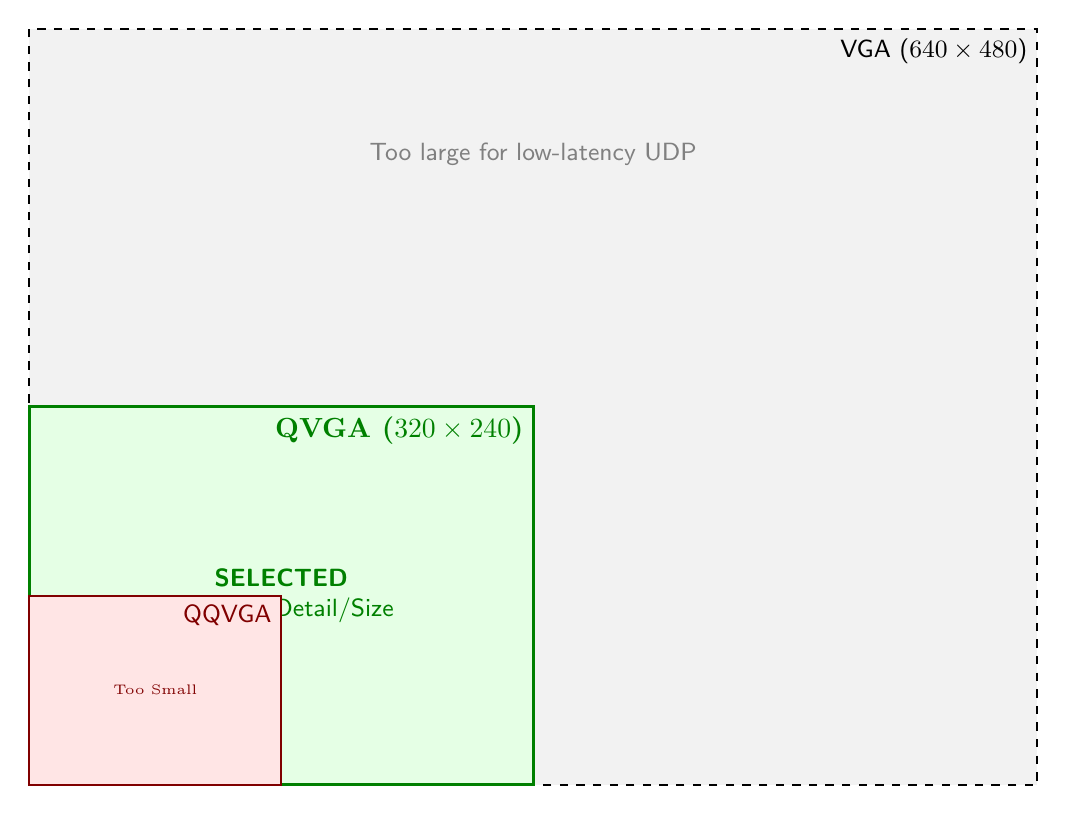
\begin{tikzpicture}[x=0.2mm, y=0.2mm, font=\sffamily\small]
        
        % Styles
        \tikzstyle{frame} = [draw=black, thick, fill=blue!5]
        \tikzstyle{label} = [fill=white, inner sep=2pt, draw=black!50]

        % VGA Frame (Reference Background)
        \draw[frame, fill=gray!10, dashed] (0,0) rectangle (640, 480);
        \node[anchor=north east] at (640, 480) {VGA ($640 \times 480$)};
        \node at (320, 400) [text=gray] {Too large for low-latency UDP};

        % QVGA Frame (Selected)
        \draw[frame, fill=green!10, draw=green!50!black, very thick] (0,0) rectangle (320, 240);
        \node[anchor=north east, text=green!50!black, font=\bfseries] at (320, 240) {QVGA ($320 \times 240$)};
        \node[align=center, text=green!50!black] at (160, 120) {\textbf{SELECTED}\\Balanced Detail/Size};

        % QQVGA Frame (Too Small)
        \draw[frame, fill=red!10, draw=red!50!black] (0,0) rectangle (160, 120);
        \node[anchor=north east, text=red!50!black] at (160, 120) {QQVGA};
        \node[text=red!50!black, font=\tiny] at (80, 60) {Too Small};

    \end{tikzpicture}
    \caption{Relative frame size comparison. The selected QVGA resolution (green) offers 4x the pixel data of QQVGA while remaining significantly smaller than VGA, fitting within the bandwidth constraints of the ESP32.}
    \label{fig:resolution-comparison}
\end{figure}

\subsection{Lens and Optical Configuration}
The system utilizes the standard lens provided with the OV2640 module. This lens features a **$65^\circ$ horizontal field of view (FOV)**. While narrower than fisheye alternatives ($120^\circ+$), this standard lens provides rectilinear images with minimal distortion, simplifying the object detection algorithms. The blind spot immediately in front of the bumper is compensated for by the downward tilt of the mounting bracket.

% FIGURE: FOV DIAGRAM
\begin{figure}[h!]
    \centering
    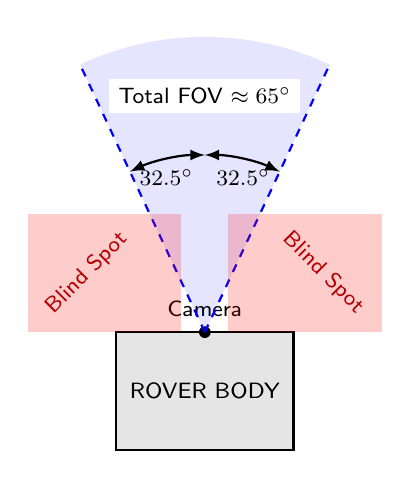
\begin{tikzpicture}[scale=0.15, >=latex, font=\sffamily\footnotesize]

        % Rover Body (Top View)
        \draw[fill=gray!20, draw=black, thick] (-7.5, -10) rectangle (7.5, 0);
        \node at (0, -5) {ROVER BODY};
        
        % Camera Position
        \node[circle, fill=black, inner sep=1.5pt] (cam) at (0, 0) {};
        \node[above] at (0,0.5) {Camera};

        % FOV Cone (65 degrees)
        \draw[blue, thick, dashed] (0,0) -- (65:25);
        \draw[blue, thick, dashed] (0,0) -- (115:25);
        
        % Fill visible area
        \fill[blue, opacity=0.1] (0,0) -- (65:25) arc (65:115:25) -- cycle;

        % Labels
        \draw[<->, thick] (0, 15) arc (90:65:15) node[midway, below] {$32.5^\circ$};
        \draw[<->, thick] (0, 15) arc (90:115:15) node[midway, below] {$32.5^\circ$};
        \node[fill=white] at (0, 20) {Total FOV $\approx 65^\circ$};

        % Blind Spots
        \fill[red, opacity=0.2] (-15,0) rectangle (-2, 10);
        \node[red!70!black, rotate=45] at (-10, 5) {Blind Spot};
        
        \fill[red, opacity=0.2] (15,0) rectangle (2, 10);
        \node[red!70!black, rotate=-45] at (10, 5) {Blind Spot};

    \end{tikzpicture}
    \caption{Field of View (FOV) coverage diagram. The standard lens provides a $65^\circ$ viewing cone. Areas outside this cone (red) are blind spots requiring the rover to rotate for full situational awareness.}
    \label{fig:camera-fov}
\end{figure}

\subsection{Camera Mounting}
The camera module is secured to the front chassis using a custom 3D-printed bracket. The mount is designed with a fixed **$15^\circ$ downward tilt**. This angle ensures that the ground is visible starting approximately $10\text{cm}$ from the front bumper, allowing the rover to detect small obstacles on the floor while maintaining visibility of the horizon.

% FIGURE: MOUNTING SIDE VIEW
\begin{figure}[h!]
    \centering
    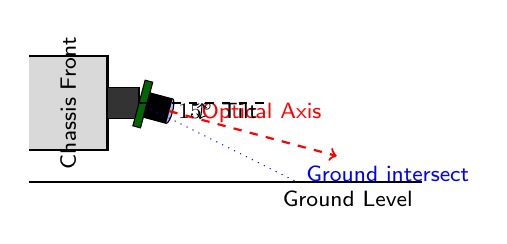
\begin{tikzpicture}[scale=0.2, font=\sffamily\footnotesize]

        % Ground
        \draw[thick] (-5, 0) -- (20, 0);
        \node[anchor=north east] at (20,0) {Ground Level};

        % Chassis Front
        \draw[fill=gray!30, draw=black, thick] (-5, 2) -- (0, 2) -- (0, 8) -- (-5, 8);
        \node[rotate=90] at (-2.5, 5) {Chassis Front};

        % Bracket
        \draw[fill=black!80] (0, 6) -- (2, 6) -- (2, 4) -- (0, 4) -- cycle;
        
        % Camera Module (Side Profile) - Tilted 15 degrees down
        % Pivot point at (2, 5)
        \begin{scope}[rotate around={-15:(2,5)}]
            % PCB
            \draw[fill=green!40!black] (2, 3.5) rectangle (2.5, 6.5);
            % Lens Barrel
            \draw[fill=black] (2.5, 4.2) rectangle (4.0, 5.8);
            % Lens Element
            \draw[fill=blue!30] (4.0, 4.2) arc (-90:90:0.2 and 0.8);
            
            % Optical Axis
            \draw[red, dashed, thick, ->] (4.0, 5) -- (15, 5);
            \node[red, above] at (10, 5.2) {Optical Axis};
        \end{scope}

        % Angle Indicator
        \draw[dashed] (2, 5) -- (10, 5); % Horizontal
        \draw[<->] (6, 5) arc (0:-15:4);
        \node at (7, 4.5) {$15^\circ$ Tilt};

        % Field of View Lines (Vertical)
        \draw[blue, dotted] (2,5) -- (12, 0); % Lower ray
        \node[blue, right] at (12, 0.5) {Ground intersect};

    \end{tikzpicture}
    \caption{Side-profile schematic of the camera mounting. The $15^\circ$ downward tilt aligns the optical axis to cover the floor surface ahead of the rover, eliminating the "under-nose" blind spot.}
    \label{fig:camera-mount}
\end{figure}

% --------------------------------------------------------
\section{Motor Control System}
\label{sec:motor-system}

The motor system provides locomotive power through two DC gear motors, one for each track. The L298N dual H-bridge driver controls motor direction and speed based on commands from the ESP32-S3.

\subsection{DC Gear Motors}

The motors are brushed DC type with integrated planetary gearboxes. The gearbox reduces output speed while increasing torque, essential for moving the chassis against friction and over obstacles.

\begin{table}[h!]
    \centering
    \caption{Motor specifications}
    \label{tab:motor-specs}
    \begin{tabular}{ll}
        \toprule
        \textbf{Parameter} & \textbf{Value} \\
        \midrule
        Nominal voltage    & 6-12V DC \\
        No-load speed      & 150 RPM at 12V \\
        Stall torque       & 3 kg-cm \\
        Stall current      & 1.5 A \\
        Operating current  & 200-500 mA \\
        Gear ratio         & 1:48 \\
        Shaft diameter     & 6 mm (D-cut) \\
        \bottomrule
    \end{tabular}
\end{table}

% FIGURE PLACEHOLDER
\begin{figure}[h!]
    \centering
    % \includegraphics[width=0.5\textwidth]{figures/hardware/dc_motor_gearbox.jpeg}
    \caption{DC gear motor showing the motor body, planetary gearbox, and output shaft.}
    \label{fig:motor-photo}
\end{figure}

\subsection{L298N Motor Driver}

The L298N is a dual full-bridge driver IC. Each bridge can deliver up to 2A continuous current, sufficient for our motors which draw 500mA under load. The module includes an onboard 5V regulator that powers the ESP32-S3.

\begin{table}[h!]
    \centering
    \caption{L298N specifications}
    \label{tab:l298n-specs}
    \begin{tabular}{ll}
        \toprule
        \textbf{Parameter} & \textbf{Value} \\
        \midrule
        Motor supply voltage & 5-35V \\
        Logic supply         & 5V (from onboard regulator or external) \\
        Per channel current  & 2A continuous, 3A peak \\
        Total power          & 25W max \\
        Control inputs       & 4 (IN1-IN4) \\
        Enable inputs        & 2 (ENA, ENB) \\
        Voltage drop         & 1.8V typical (at rated current) \\
        \bottomrule
    \end{tabular}
\end{table}

% FIGURE PLACEHOLDER
\begin{figure}[h!]
    \centering
    \includegraphics[width=0.6\textwidth]{figures/hardware/l298n_module.jpeg}
    \caption{L298N motor driver module with the characteristic large heatsink and terminal blocks.}
    \label{fig:l298n-module}
\end{figure}

\subsection{L298N vs TB6612FNG}

During component selection, we compared the L298N against the more modern TB6612FNG. The TB6612 offers higher efficiency (90\% vs 70\%) due to MOSFET switching rather than bipolar transistors. However, the L298N was selected because of its higher current capacity and integrated voltage regulator.

\begin{table}[h!]
    \centering
    \caption{Motor driver comparison}
    \label{tab:driver-comparison}
    \begin{tabular}{lcc}
        \toprule
        \textbf{Feature} & \textbf{L298N} & \textbf{TB6612FNG} \\
        \midrule
        Max current     & 2A    & 1.2A \\
        Efficiency      & 70\%  & 90\% \\
        Voltage drop    & 1.8V  & 0.3V \\
        Heat generation & High  & Low \\
        5V regulator    & Built-in & None \\
        Cost            & \$3   & \$5 \\
        Selected        & Yes   & No \\
        \bottomrule
    \end{tabular}
\end{table}

The lower efficiency of the L298N means more power is dissipated as heat. For extended operation, the heatsink temperature can exceed 60 degrees Celsius. Future revisions may switch to the TB6612 if thermal throttling becomes problematic.

% FIGURE PLACEHOLDER
\begin{figure}[h!]
    \centering
    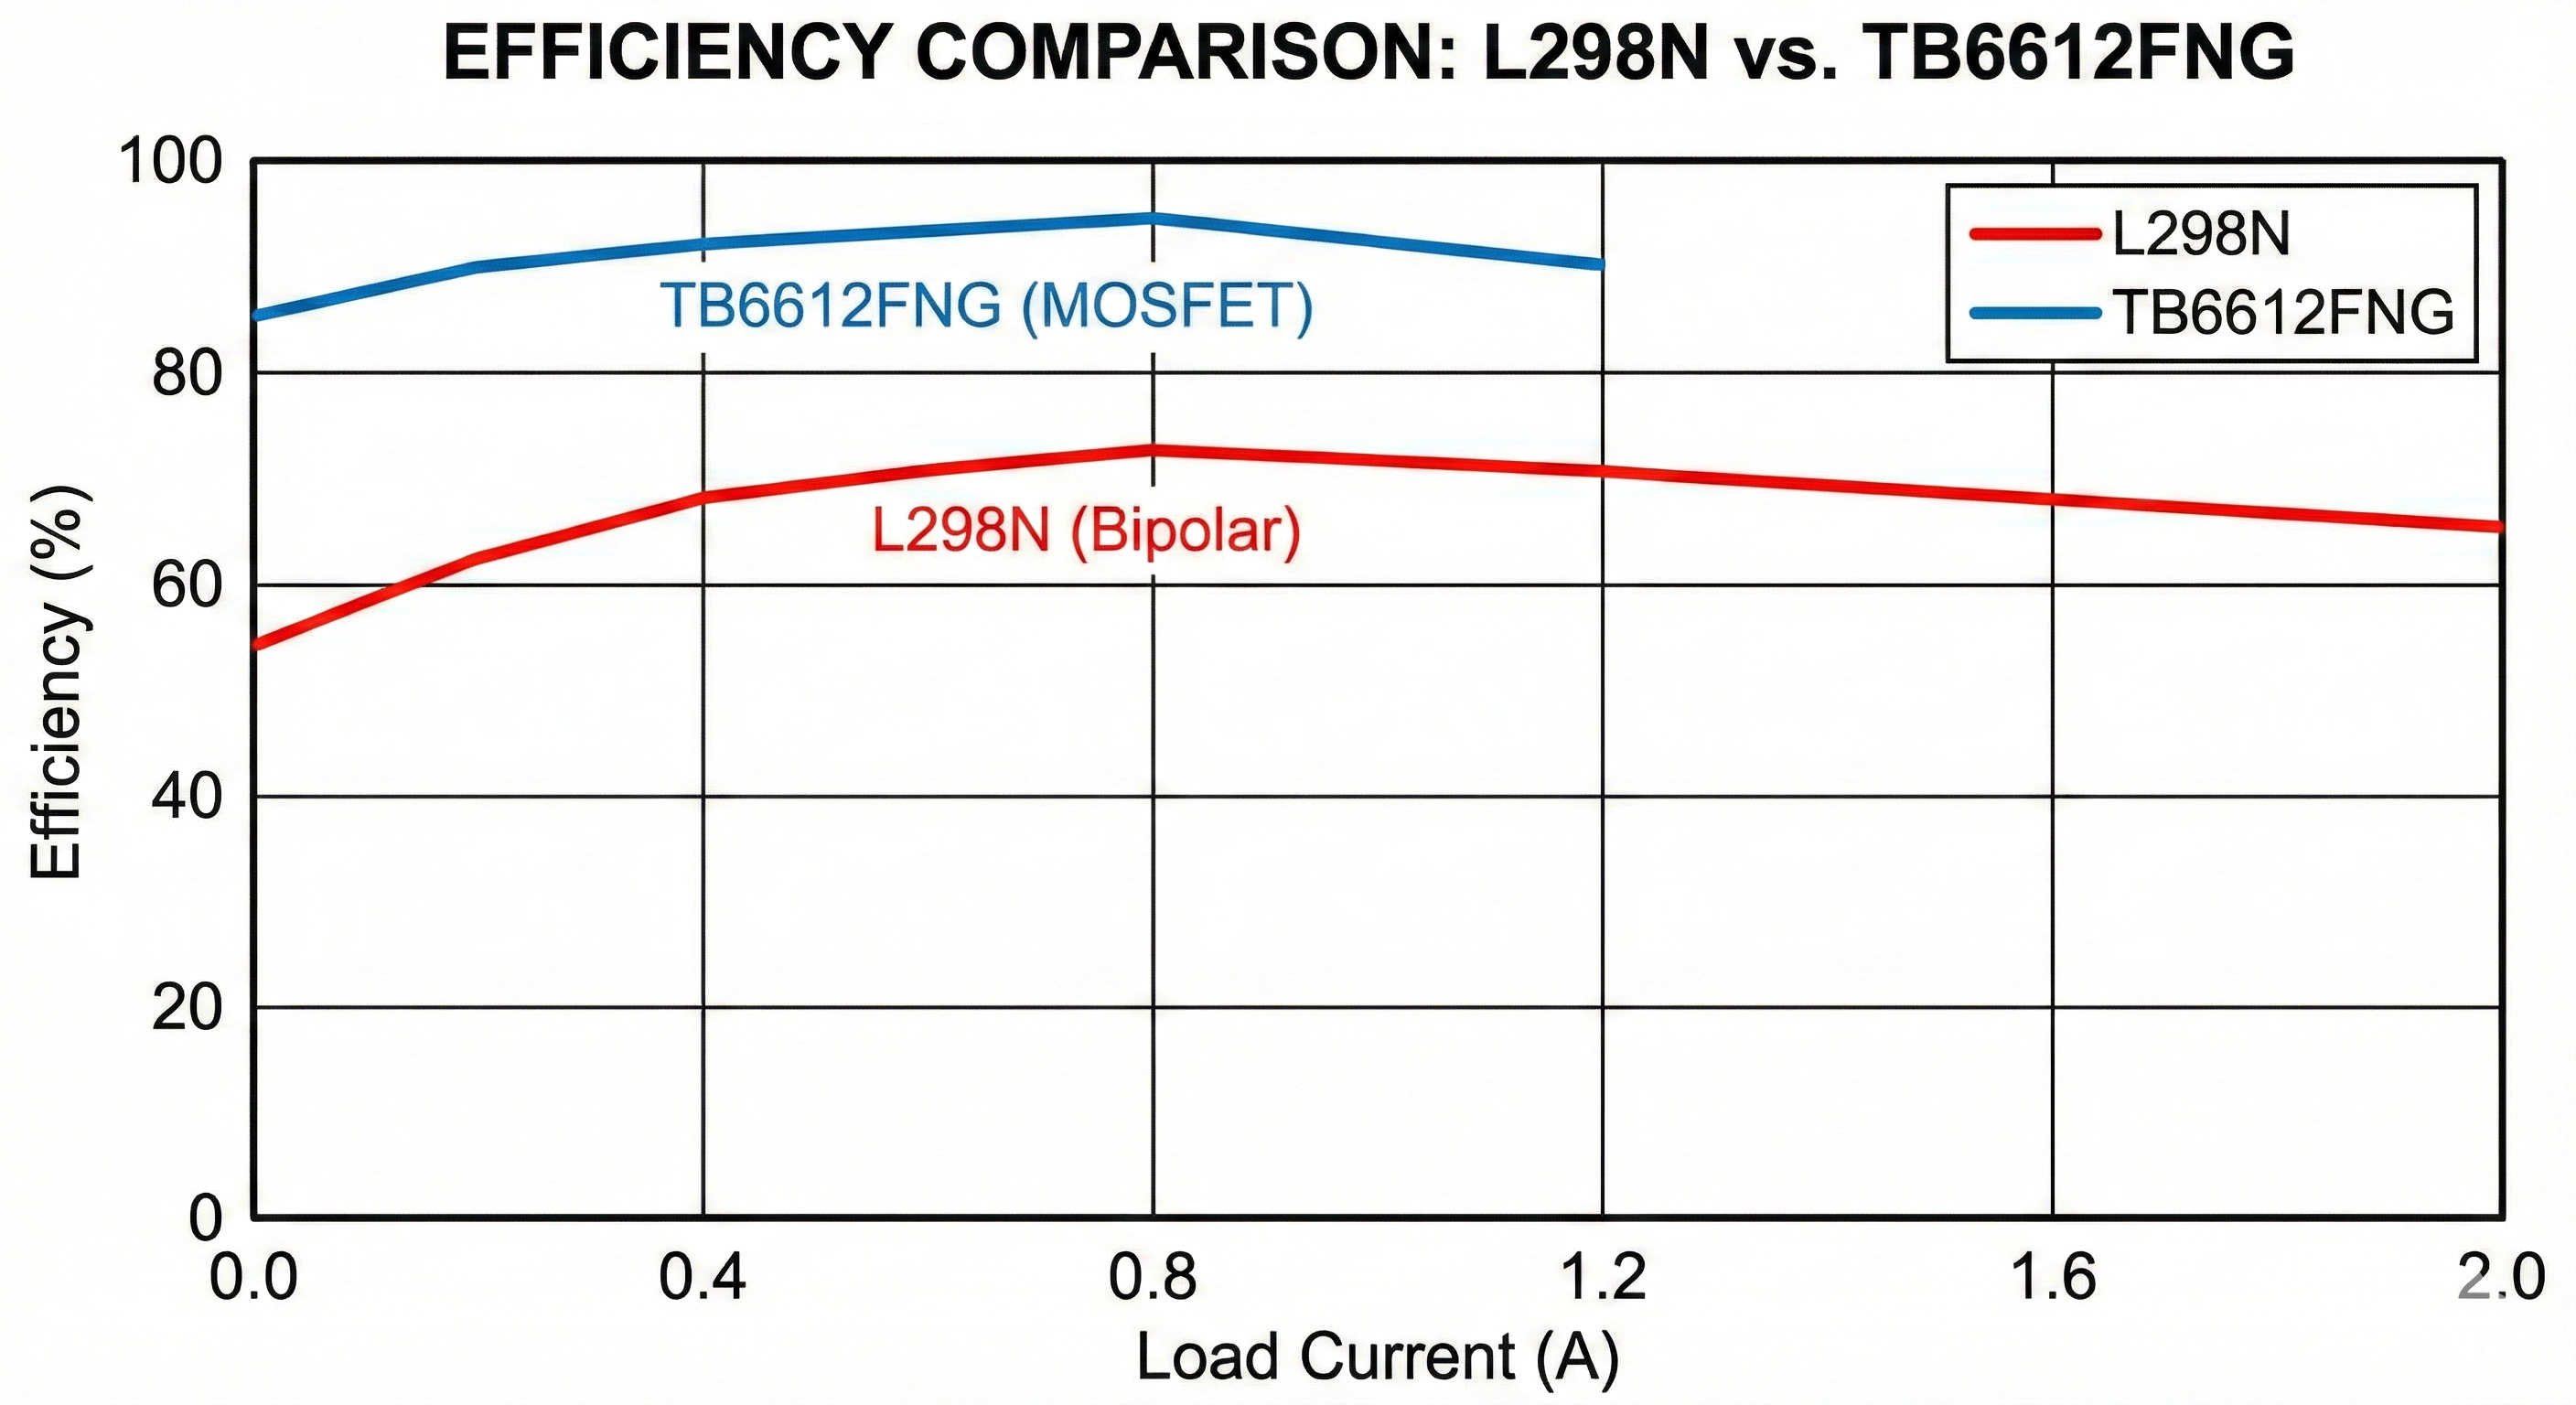
\includegraphics[width=0.8\textwidth]{figures/charts/driver_efficiency.png}
    \label{fig:efficiency-graph}
\end{figure}

% --------------------------------------------------------
\section{Power Distribution}
\label{sec:power-distribution}

The power system delivers appropriate voltages to all components from a single lithium polymer battery. Power management includes voltage regulation, protection circuits, and monitoring.

\subsection{Battery Selection}

A 3-cell (3S) lithium polymer battery provides the primary power. The 11.1V nominal voltage is compatible with both the motors (rated for 6-12V) and the L298N 5V regulator input range.

\begin{table}[h!]
    \centering
    \caption{Battery specifications}
    \label{tab:battery-specs}
    \begin{tabular}{ll}
        \toprule
        \textbf{Parameter} & \textbf{Value} \\
        \midrule
        Chemistry       & Lithium Polymer (LiPo) \\
        Configuration   & 3S (3 cells in series) \\
        Nominal voltage & 11.1V \\
        Fully charged   & 12.6V \\
        Low cutoff      & 9.9V (3.3V per cell) \\
        Capacity        & 2200 mAh \\
        Discharge rate  & 25C continuous \\
        Weight          & 180g \\
        \bottomrule
    \end{tabular}
\end{table}

% FIGURE PLACEHOLDER
\begin{figure}[H]
    \centering
    \includegraphics[width=0.5\textwidth]{figures/hardware/lipo_battery.jpeg}
    \caption{3S LiPo battery used to power the Rescue Rover.}
    \label{fig:battery-photo}
\end{figure}

\subsection{Power Budget}

The power budget analysis ensures the battery can supply all loads simultaneously. Total maximum draw is approximately 2.5A, well within the battery's 55A (25C x 2.2Ah) capability.

\begin{table}[h!]
    \centering
    \caption{System power budget}
    \label{tab:power-budget}
    \begin{tabular}{lccc}
        \toprule
        \textbf{Component} & \textbf{Voltage} & \textbf{Current (typ)} & \textbf{Current (max)} \\
        \midrule
        ESP32-S3 + Camera & 3.3V  & 300 mA  & 500 mA \\
        L298N quiescent   & 5V    & 36 mA   & 50 mA \\
        Left motor        & 12V   & 250 mA  & 1.5 A \\
        Right motor       & 12V   & 250 mA  & 1.5 A \\
        Ultrasonic sensor & 5V    & 15 mA   & 20 mA \\
        \midrule
        \textbf{Total}    & --    & 851 mA  & 3.57 A \\
        \bottomrule
    \end{tabular}
\end{table}

At typical consumption of 851 mA, the 2200 mAh battery provides approximately 2.5 hours of operation. Under maximum load (both motors stalled), runtime drops to approximately 40 minutes. Actual runtime during normal operation falls between these extremes.

% FIGURE PLACEHOLDER
\begin{figure}[H]
    \centering
    \includegraphics[width=\textwidth]{figures/hardware/power_distribution_diagram.png}
    \caption{Power distribution schematic showing voltage rails and current flow to all components.}
    \label{fig:power-schematic}
\end{figure}

\subsection{Voltage Regulation}

The L298N module includes a 78M05 linear regulator that provides 5V output from the 12V motor supply. This 5V rail powers the ESP32-S3 and ultrasonic sensor. The ESP32's internal LDO then produces 3.3V for the microcontroller core and camera.

% FIGURE PLACEHOLDER
\begin{figure}[H]
    \centering
    \includegraphics[width=\textwidth]{figures/hardware/voltage_rails.png}
    \caption{Voltage rail hierarchy showing the cascade of regulators from battery to components.}
    \label{fig:voltage-rails}
\end{figure}

% --------------------------------------------------------
\section{Ultrasonic Distance Sensor}
\label{sec:ultrasonic-sensor}

The ultrasonic sensor provides proximity detection for obstacle avoidance. It measures the time of flight for a sound pulse to reach an obstacle and return.

\subsection{HC-SR04 Specifications}

\begin{table}[h!]
    \centering
    \caption{Ultrasonic sensor specifications}
    \label{tab:hcsr04-specs}
    \begin{tabular}{ll}
        \toprule
        \textbf{Parameter} & \textbf{Value} \\
        \midrule
        Operating voltage  & 5V DC \\
        Operating current  & 15 mA \\
        Frequency          & 40 kHz \\
        Range              & 2 cm to 400 cm \\
        Resolution         & 0.3 cm \\
        Measuring angle    & 15 degrees cone \\
        Trigger pulse      & 10 $\mu$s minimum \\
        \bottomrule
    \end{tabular}
\end{table}

% FIGURE PLACEHOLDER
\begin{figure}[H]
    \centering
    \includegraphics[width=0.5\textwidth]{figures/hardware/hcsr04_photo.jpeg}
    \caption{HC-SR04 ultrasonic distance sensor showing the transmitter and receiver transducers.}
    \label{fig:hcsr04-photo}
\end{figure}

\subsection{Mounting Position}

The sensor is mounted at the front of the chassis, below the camera. This position provides distance measurements along the rover's direction of travel. The narrow 15-degree beam angle means only obstacles directly ahead are detected. Side obstacles require camera based detection.

% FIGURE: ULTRASONIC BEAM PATTERN
\begin{figure}[H]
    \centering
    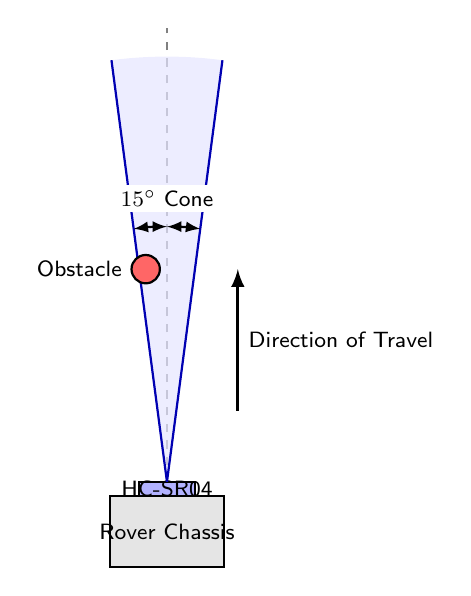
\begin{tikzpicture}[scale=0.18, >=latex, font=\sffamily\footnotesize]
        % Rover Chassis (Top View)
        \draw[fill=gray!20, thick] (-4, -5) rectangle (4, 0);
        \node at (0, -2.5) {Rover Chassis};

        % Ultrasonic Sensor (mounted at the front)
        \draw[fill=blue!30, thick] (-2, 0) rectangle (2, 1);
        \node at (0, 0.5) {HC-SR04};

        % Beam Cone (15 degrees total -> +/- 7.5 degrees from center)
        \begin{scope}[shift={(0,1)}]
            % Center line
            \draw[dashed, gray, thin] (0,0) -- (0,32);

            % Cone area
            \fill[blue!10, opacity=0.7] (0,0) -- (97.5:30) arc (97.5:82.5:30) -- cycle;
            % Cone edges
            \draw[blue!70!black, thick] (0,0) -- (97.5:30);
            \draw[blue!70!black, thick] (0,0) -- (82.5:30);

            % Angle Label
            \draw[<->, thick] (0, 18) arc (90:97.5:18);
            \draw[<->, thick] (0, 18) arc (90:82.5:18);
            \node[fill=white, inner sep=2pt] at (0, 20) {$15^\circ$ Cone};

            % Example Obstacle
            \draw[fill=red!60, thick] (-1.5, 15) circle (1);
            \node[left] at (-2.5, 15) {Obstacle};
            
            % Direction Arrow
            \draw[->, thick, very thick] (5, 5) -- (5, 15) node[midway, right] {Direction of Travel};
        \end{scope}
    \end{tikzpicture}
    \caption{Top-down view of the ultrasonic sensor's beam pattern. The narrow $15^\circ$ detection cone is shown relative to the rover chassis, detecting obstacles directly ahead.}
    \label{fig:ultrasonic-beam}
\end{figure}

\subsection{Level Shifting}

The HC-SR04 operates at 5V logic levels while the ESP32-S3 GPIO pins are 3.3V. The echo pin outputs 5V, which could damage the ESP32 input. A simple resistor voltage divider scales the echo signal down to 3.3V safe levels.

\begin{lstlisting}[caption={Voltage divider calculation}]
R1 = 1kOhm, R2 = 2kOhm
V_out = V_in * R2 / (R1 + R2)
V_out = 5V * 2k / 3k = 3.33V
\end{lstlisting}

% FIGURE PLACEHOLDER
\begin{figure}[H]
    \centering
    \includegraphics[width=0.6\textwidth]{figures/hardware/level_shifter_circuit.png}
    \caption{Resistor voltage divider for level shifting the 5V echo signal to 3.3V.}
    \label{fig:level-shifter}
\end{figure}

% --------------------------------------------------------
\section{Wiring and Interconnections}
\label{sec:wiring}

This section documents all electrical connections between components. Dupont jumper wires are used throughout for easy modification during development.

\subsection{Complete Wiring Diagram}

% FIGURE PLACEHOLDER
\begin{figure}[H]
    \centering
    \includegraphics[width=\textwidth]{figures/hardware/complete_wiring_diagram.jpg}
    \caption{Complete wiring diagram showing all connections between the ESP32-S3, L298N, motors, sensors, and power supply.}
    \label{fig:complete-wiring}
\end{figure}

\subsection{Wire Color Convention}

\begin{table}[h!]
    \centering
    \caption{Wire color coding standard}
    \label{tab:wire-colors}
    \begin{tabular}{ll}
        \toprule
        \textbf{Color} & \textbf{Purpose} \\
        \midrule
        Red    & Positive power (12V, 5V, 3.3V) \\
        Black  & Ground \\
        Yellow & Signal (GPIO outputs) \\
        Orange & Signal (GPIO inputs) \\
        Green  & I2C SDA \\
        Blue   & I2C SCL \\
        \bottomrule
    \end{tabular}
\end{table}

% FIGURE PLACEHOLDER
\begin{figure}[H]
    \centering
    \includegraphics[width=\textwidth]{figures/hardware/wiring_photo.jpg}
    \caption{Actual wiring on the prototype showing careful routing and color coding.}
    \label{fig:wiring-photo}
\end{figure}

% --------------------------------------------------------
\section{Assembly Process}
\label{sec:assembly}

The complete assembly follows a specific order to ensure proper fit and cable routing.

\subsection{Assembly Steps}

\begin{enumerate}
    \item Mount motors to chassis brackets using M3 screws
    \item Attach drive sprockets to motor shafts
    \item Install tracks with proper tension
    \item Mount battery holder to rear platform
    \item Attach L298N driver with standoffs
    \item Mount ESP32-S3 board adjacent to L298N
    \item Install ultrasonic sensor at front
    \item Mount camera module on adjustable bracket
    \item Complete all wiring connections
    \item Verify connections with multimeter before power on
\end{enumerate}

% FIGURE PLACEHOLDER
\begin{figure}[H]
    \centering
    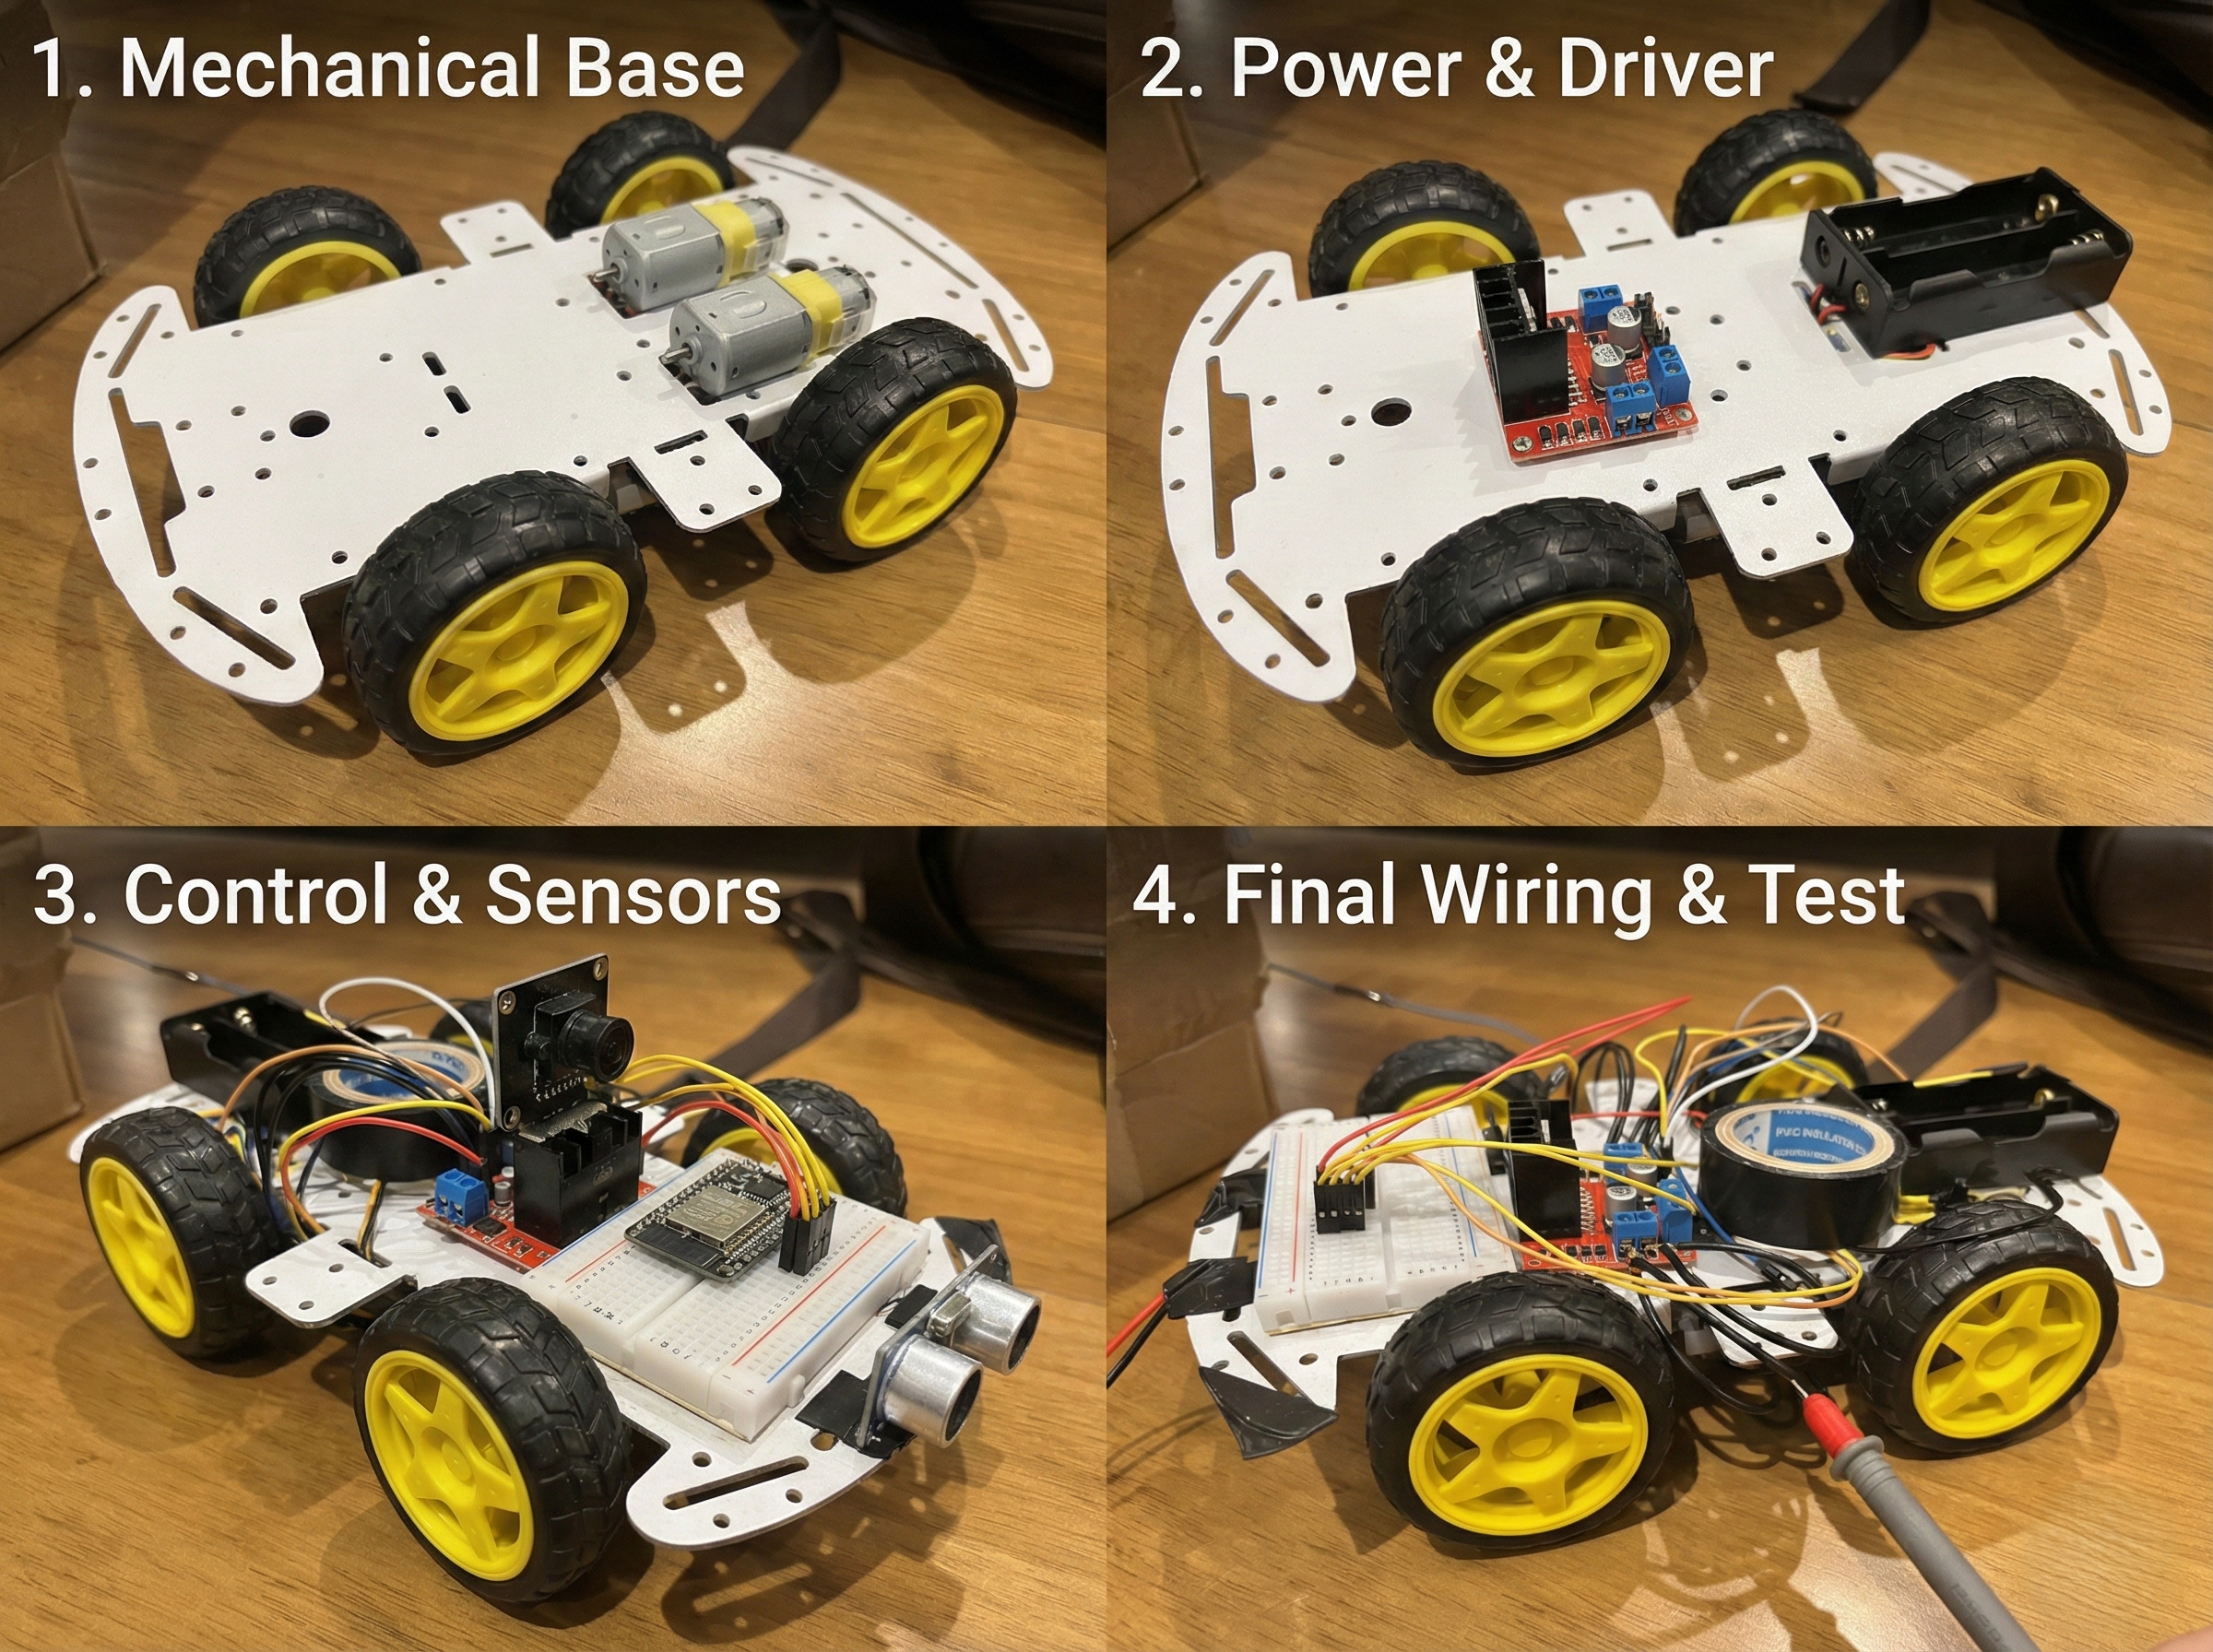
\includegraphics[width=\textwidth]{figures/hardware/assembly_sequence.png}
    \caption{Assembly sequence showing the progressive addition of components to the chassis.}
    \label{fig:assembly-sequence}
\end{figure}

\subsection{Testing Procedure}

After assembly, each subsystem is tested individually before full integration testing.

\begin{table}[h!]
    \centering
    \caption{Post-assembly test checklist}
    \label{tab:test-checklist}
    \begin{tabular}{lp{8cm}}
        \toprule
        \textbf{Subsystem} & \textbf{Test Procedure} \\
        \midrule
        Power     & Verify 5V and 3.3V rails with multimeter \\
        Motors    & Check rotation direction for each motor separately \\
        Camera    & Verify video feed appears in browser \\
        Ultrasonic & Move hand toward sensor, verify distance changes \\
        WiFi      & Confirm connection to access point \\
        ESP-NOW   & Verify command reception from gateway \\
        \bottomrule
    \end{tabular}
\end{table}

% FIGURE PLACEHOLDER
\begin{figure}[H]
    \centering
    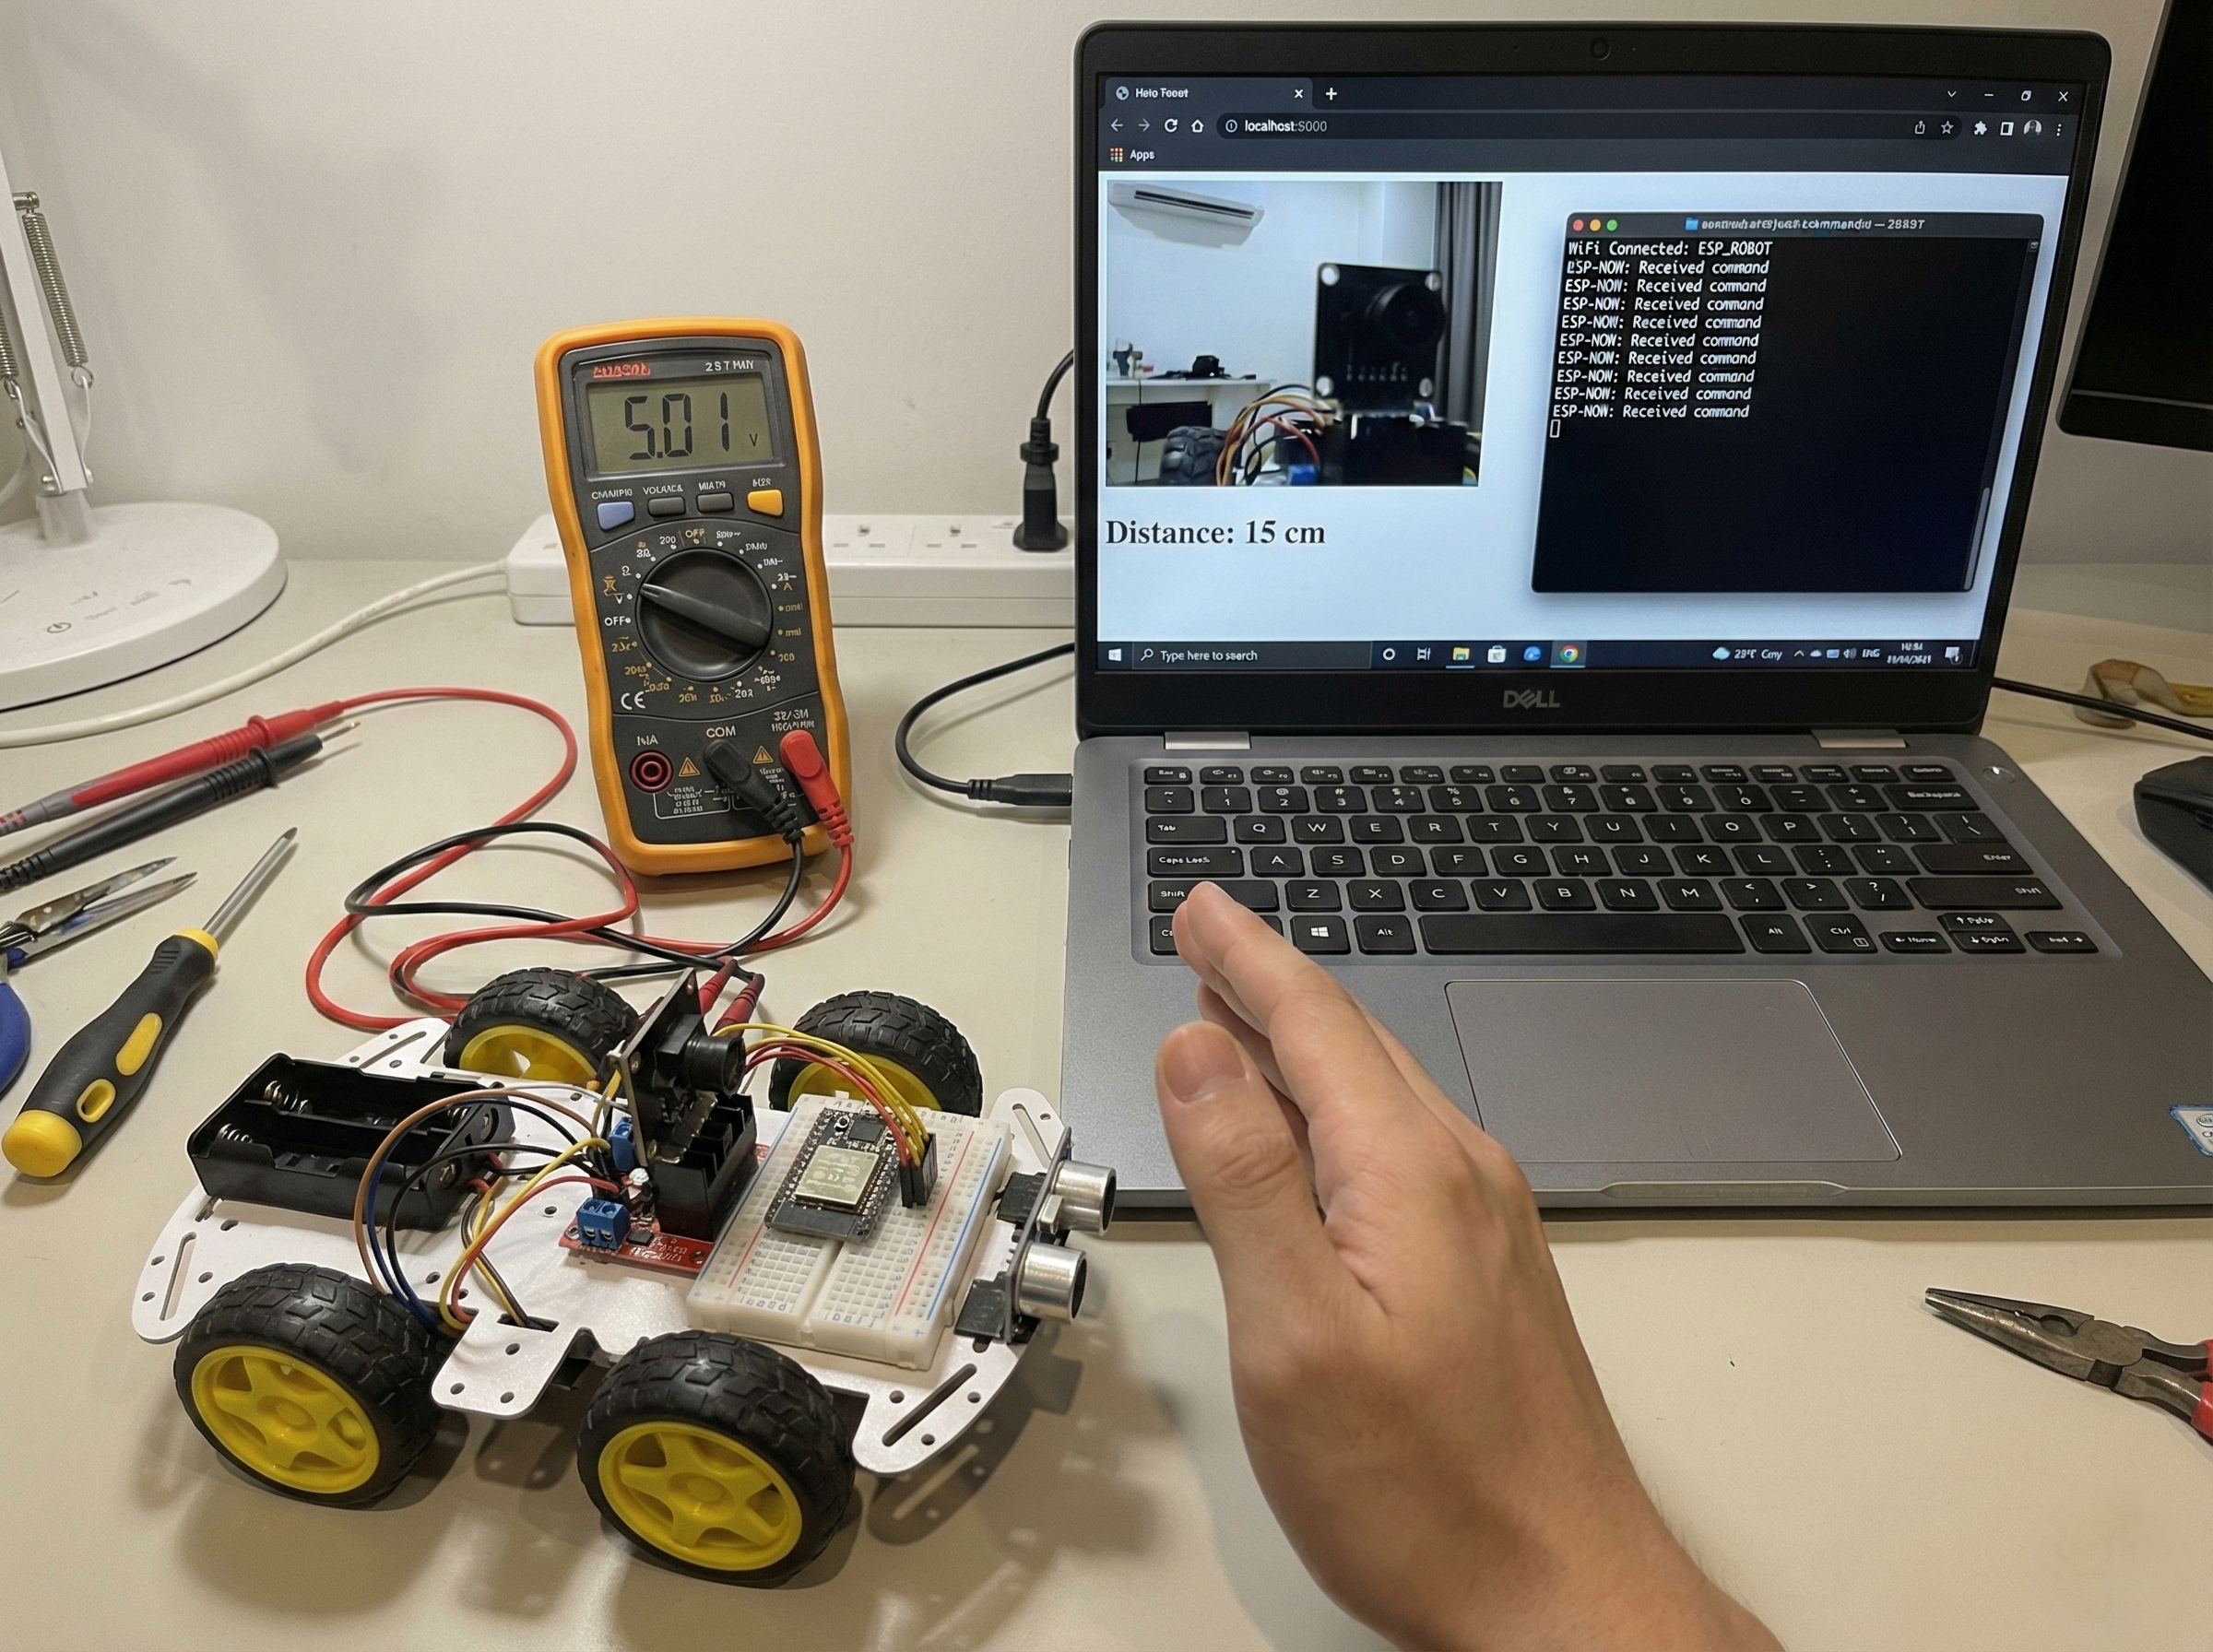
\includegraphics[width=\textwidth]{figures/hardware/testing_setup.png}
    \caption{Testing setup for post-assembly verification of subsystems.}
    \label{fig:testing-setup}
\end{figure}
